\documentclass[a4paper]{article}
\usepackage{vntex}
%\usepackage[english,vietnam]{babel}
%\usepackage[utf8]{inputenc}

%\usepackage[utf8]{inputenc}
%\usepackage[francais]{babel}
\usepackage{a4wide,amssymb,epsfig,latexsym,array,hhline,fancyhdr}

\usepackage{amsmath}
\usepackage{amsthm}
\usepackage{multicol,longtable,amscd}
\usepackage{diagbox}%Make diagonal lines in tables
\usepackage{booktabs}
\usepackage{alltt}
\usepackage[framemethod=tikz]{mdframed}% For highlighting paragraph backgrounds
\usepackage{caption,subcaption}

\usepackage{lastpage}
\usepackage[lined,boxed,commentsnumbered]{algorithm2e}
\usepackage{enumerate}
\usepackage{color}
\usepackage{graphicx}							% Standard graphics package
\usepackage{array}
\usepackage{tabularx, caption}
\usepackage{multirow}
\usepackage{multicol}
\usepackage{rotating}
\usepackage{graphics}
\usepackage{geometry}
\usepackage{setspace}
\usepackage{epsfig}
\usepackage{tikz}
\usetikzlibrary{arrows,snakes,backgrounds}
\usepackage[unicode]{hyperref}
\hypersetup{urlcolor=blue,linkcolor=black,citecolor=black,colorlinks=true} 
%\usepackage{pstcol} 								% PSTricks with the standard color package

\usepackage{graphicx}
\usepackage{xcolor}
\usepackage{dirtree}
% The following is a dummy icon command
\newcommand\myicon[1]{{\color{#1}\rule{2ex}{2ex}}}
% If you have actual icon images, use \includegraphics to include them
% If you are generating them, put in the appropriate code for them here
% now we make a command for a folder/file which inserts the icon and its label
% adjust this as needed. If you only have 2 icons, then you could create
% a \myfile and \myfolder command with the icon fixed.
\newcommand{\myfolder}[2]{\myicon{#1}\ {#2}}




%\usepackage{fancyhdr}
\setlength{\headheight}{40pt}
\pagestyle{fancy}
\fancyhead{} % clear all header fields
\fancyhead[L]{
 \begin{tabular}{rl}
    \begin{picture}(25,15)(0,0)
    \put(0,-8){
\includegraphics[width=8mm, height=8mm]{Images/hcmut.png}}
    %\put(0,-8){\epsfig{width=10mm,figure=hcmut.eps}}
   \end{picture}&
	%
\includegraphics[width=8mm, height=8mm]{hcmut.png} & %
	\begin{tabular}{l}
		\textbf{\bf \ttfamily Trường Đại Học Bách Khoa Tp.Hồ Chí Minh}\\
		\textbf{\bf \ttfamily Khoa Khoa Học và Kỹ Thuật Máy Tính}
	\end{tabular} 	
 \end{tabular}
}
\fancyhead[R]{
	\begin{tabular}{l}
		\tiny \bf \\
		\tiny \bf 
	\end{tabular}  }
\fancyfoot{} % clear all footer fields
\fancyfoot[R]{\scriptsize \ttfamily Trang {\thepage}/\pageref{LastPage}}
\renewcommand{\headrulewidth}{0.3pt}
\renewcommand{\footrulewidth}{0.3pt}


%%%
\setcounter{secnumdepth}{4}
\setcounter{tocdepth}{3}
\makeatletter
\newcounter {subsubsubsection}[subsubsection]
\renewcommand\thesubsubsubsection{\thesubsubsection .\@alph\c@subsubsubsection}
\newcommand\subsubsubsection{\@startsection{subsubsubsection}{4}{\z@}%
                                     {-3.25ex\@plus -1ex \@minus -.2ex}%
                                     {1.5ex \@plus .2ex}%
                                     {\normalfont\normalsize\bfseries}}
\newcommand*\l@subsubsubsection{\@dottedtocline{3}{10.0em}{4.1em}}
\newcommand*{\subsubsubsectionmark}[1]{}
\makeatother

\everymath{\color{blue}}%make in-line maths symbols blue to read/check easily

\sloppy
\captionsetup[figure]{labelfont={small,bf},textfont={small,it},belowskip=-1pt,aboveskip=-9pt}
%space remove between caption, figure, and text
\captionsetup[table]{labelfont={small,bf},textfont={small,it},belowskip=-1pt,aboveskip=7pt}
%space remove between caption, table, and text

%\floatplacement{figure}{H}%forced here float placement automatically for figures
%\floatplacement{table}{H}%forced here float placement automatically for table
%the following settings (11 lines) are to remove white space before or after the figures and tables
%\setcounter{topnumber}{2}
%\setcounter{bottomnumber}{2}
%\setcounter{totalnumber}{4}
%\renewcommand{\topfraction}{0.85}
%\renewcommand{\bottomfraction}{0.85}
%\renewcommand{\textfraction}{0.15}
%\renewcommand{\floatpagefraction}{0.8}
%\renewcommand{\textfraction}{0.1}
\setlength{\floatsep}{5pt plus 2pt minus 2pt}
\setlength{\textfloatsep}{5pt plus 2pt minus 2pt}
\setlength{\intextsep}{10pt plus 2pt minus 2pt}

\begin{document}

\begin{titlepage}
\begin{center}
ĐẠI HỌC QUỐC GIA THÀNH PHỐ HỒ CHÍ MINH \\
TRƯỜNG ĐẠI HỌC BÁCH KHOA \\
KHOA KHOA HỌC - KỸ THUẬT MÁY TÍNH 
\end{center}

\vspace{1cm}

\begin{figure}[h!]
\begin{center}

\includegraphics[width=4cm]{Images/hcmut.png}
\end{center}
\end{figure}

\vspace{1cm}


\begin{center}
\begin{tabular}{c}
\multicolumn{1}{c}{\textbf{{\Huge MẠNG MÁY TÍNH}}}\\
~~\\
\hline
\\
\multicolumn{1}{l}{\textbf{{\Large Bài tập lớn}}}\\
\multicolumn{1}{l}{\textbf{{\Large Nhóm: 103 --- Lớp: L05}}}\\
\\
\textbf{{\Huge Xây dựng ứng dụng chat với}} \\
\textbf{{\Huge WebSocket bằng Django và ReacJS}}\\
\\
\hline
\end{tabular}
\end{center}

\vspace{0.75cm}

\begin{table}[h]
\begin{tabular}{rrl}
\hspace{5 cm} & GVHD: & Bùi Xuân Giang \\
& SV thực hiện: & Huỳnh Quốc Phú -- 1712638 \\
& 				& Nguyễn Duy Nguyên -- 1712380 \\
& 				& Trần Mạnh Hưng -- 1711646 \\
\end{tabular}
\end{table}
\vspace{1.5cm}
\begin{center}
{\footnotesize Tp. Hồ Chí Minh, Tháng 11/2019}
\end{center}
\end{titlepage}


%\thispagestyle{empty}

\newpage
\tableofcontents
\listoffigures
\newpage
Bài báo cáo là tổng hợp của hai giai đoạn theo đặc tả của bài tập lớn.

Phần đầu là giai đoạn một với nội dung là định các chức năng của ứng dụng và định nghĩa các giao thức sử dụng trong ứng dụng.

Phần thứ hai gồm các miêu tả chi tiết các chức năng đã thực hiện, về kiến trúc của ứng dụng kèm theo đó là các đánh giá của nhóm và source code của ứng dụng.

%%%%%%%%%%%%%%%%%%%%%%%%%%%%%%%%%
\section{Giai đoạn một}\label{giai_doan_1}
	\subsection{Tổng quan về các chức năng của ứng dụng}
	Dựa trên các yêu cầu của bài tập lớn, nhóm đề xuất các chức năng chính cần có của ứng dụng như sau:
		\begin{itemize}
			\item Hệ thống định danh người dùng : Đăng nhập, đăng suất, lưu thông tin người dùng để định danh phân biệt giữa các người dùng trong hệ thống.
			\item Hệ thống trò chuyện : Có thể trò chuyện giữa hai người với nhau, lưu lại lịch sử trò chuyện cũng như mốc thời gian của tin nhắn.
			\item Hệ thống tạo cuộc trò chuyện : Có thể tạo một cuộc trò chuyện mới với các người dùng khác trong cùng hệ thống.
			\item Hệ thống xác định trạng thái : Xác định trạng thái hoạt động của một người dùng trong hệ thống.
			\item Hệ thống gửi file và ảnh : trong cuộc trò chuyện có thể gửi thêm kèo theo file hay ảnh đính kèm.
		\end{itemize}
	\subsection{Các giao thức sử dụng cho từng chức năng}
	Đối với các chức năng đã được định nghĩa ở trên, nhóm đưa ra đề suất xử dụng hai giao thức chính để hoàn chỉnh các tác vụ trên như sau : 
		% 2.1
		\subsubsection{WebSocket : }
		Websocket là giao thức hỗ trợ giao tiếp hai chiều giữa client và server để tạo một kết nối trao đổi dữ liệu. Sử dụng TCP, để loại bỏ vấn đề thời hạn kết .\\
		Giao thức WebSocket là một giao thức được sử dụng rộng rãi cho việc phát triển ứng dụng real-time do việc cung cấp giao thức giao tiếp hai chiều mạnh mẽ, có độ trễ thấp và dễ xử lý lỗi.\\\\
		Các gói tin (packets) của Websocket nhẹ hơn HTTP rất nhiều. Nó giúp giảm độ trễ của network nhiều lần.\\
		Cấu trúc của Websoket được thể hiện như hình sau : 
			\begin{center}
					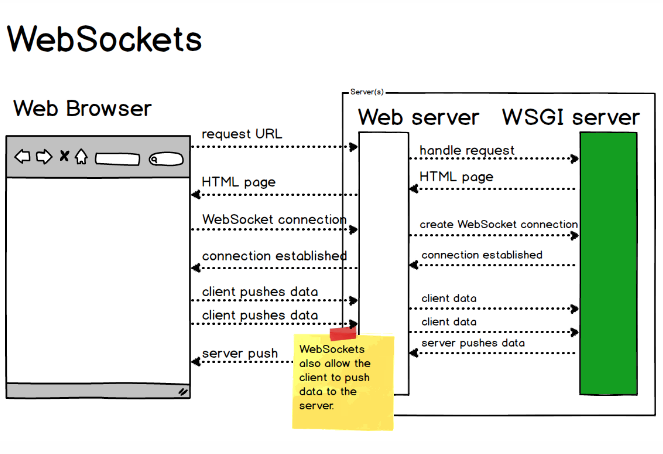
\includegraphics[scale=0.7]{Images/websocket.png}
					\captionof{figure}{Cấu trúc của một Websocket.}
			\end{center}
		\text{}\\
		\textbf{WebSocket được sử dụng trong ứng dụng để hiện thực hệ thống Chat giữa người dùng với nhau và cả hệ thống gửi file và ảnh.}\\
		
		% 2.2
		\subsubsection{REST API : }
		RESTful API là một tiêu chuẩn dùng trong việc thiết kế API cho các ứng dụng web (thiết kế Web services) để tiện cho việc quản lý các resource. Nó chú trọng vào tài nguyên hệ thống (tệp văn bản, ảnh, âm thanh, video, hoặc dữ liệu động…), bao gồm các trạng thái tài nguyên được định dạng và được truyền tải qua HTTP. \\\\
		API (Application Programming Interface) là một tập các quy tắc và cơ chế mà theo đó, một ứng dụng hay một thành phần sẽ tương tác với một ứng dụng hay thành phần khác. API có thể trả về dữ liệu mà bạn cần cho ứng dụng của mình ở những kiểu dữ liệu phổ biến như JSON hay XML. Ở ứng dụng này, nhóm sử dụng JSON. \\\\
		REST (REpresentational State Transfer) là một dạng chuyển đổi cấu trúc dữ liệu, một kiểu kiến trúc để viết API. Nó sử dụng phương thức HTTP đơn giản để tạo cho giao tiếp giữa các máy. Vì vậy, thay vì sử dụng một URL cho việc xử lý một số thông tin người dùng, REST gửi một yêu cầu HTTP như GET, POST, DELETE, vv đến một URL để xử lý dữ liệu.\\\\
		Chức năng quan trọng nhất của REST là quy định cách sử dụng các HTTP method (như GET, POST, PUT, DELETE…) và cách định dạng các URL cho ứng dụng web để quản các resource. RESTful không quy định logic code ứng dụng và không giới hạn bởi ngôn ngữ lập trình ứng dụng, bất kỳ ngôn ngữ hoặc framework nào cũng có thể sử dụng để thiết kế một RESTful API.\\\\	
		Hoạt động của REST API được thể hiện như hình sau :
			\begin{center}
				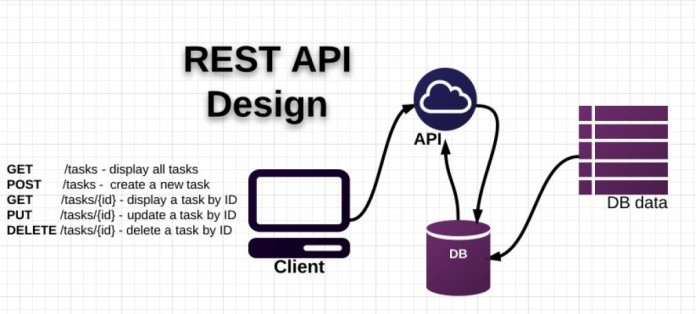
\includegraphics[scale=0.7]{Images/restfulapi.jpg}
				\captionof{figure}{Hoạt động của một RESTful API.}
			\end{center}
		\text{}\\
		\textbf{REST API được sử dụng trong ứng dụng để hiện thực hệ thống định danh người dùng cùng với đó là hệ thống duyệt và tạo các cuộc trò chuyện.}\\
		


	

%%%%%%%%%%%%%%%%%%%%%%%%%%%%%%%%%
\section{Giao đoạn hai}\label{giai_doan_2}
Trong phần này nhóm sẽ trình bày chi tiết về các chức năng,về kiến trúc của ứng dụng và tự đánh giá quá trình làm việc của từng cá nhân trong nhóm. 
	\subsection{Chi tiết các chứng năng của ứng dụng}  
	\begin{itemize}
		\item \textbf{Hệ thống định danh người dùng :} \\
		Đăng nhập, đăng ký và đăng suất được dựa trên cơ chế REST framework trong django và được hiện thực như hình sau : 
			\begin{center}
					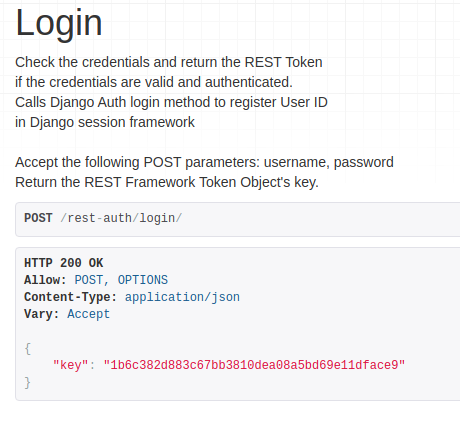
\includegraphics[scale=0.7]{Images/login.png}
					\captionof{figure}{Cơ chế Login}
					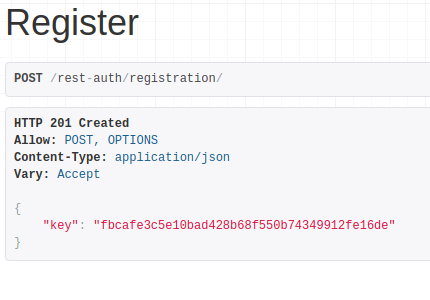
\includegraphics[width=.6\linewidth]{Images/signup.png}
					\captionof{figure}{Cơ chế SignUp}
			\end{center}
		Thông tin người dùng được lưu trên DataBase như sau : 
			\begin{center}
				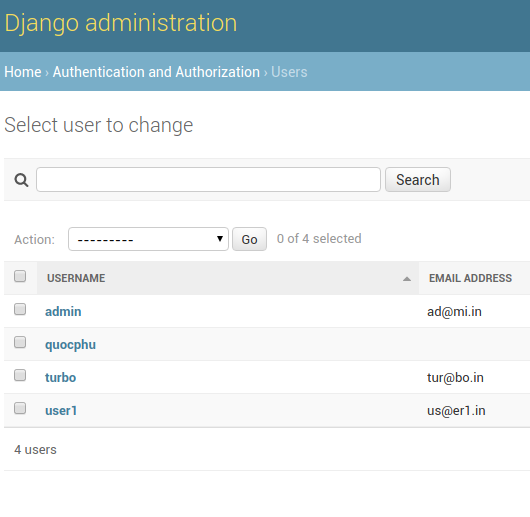
\includegraphics[scale=0.7]{Images/userdata.png}
				\captionof{figure}{Dữ liệu được lưu chia thành User/SuperUser}
			\end{center}
		
		\item \textbf{Hệ thống trò chuyện :} \\
		Có thể trò chuyện giữa hai người với nhau, lưu lại lịch sử trò chuyện cũng như mốc thời gian của tin nhắn. Được thể hiện như sau : 
			\begin{center}
				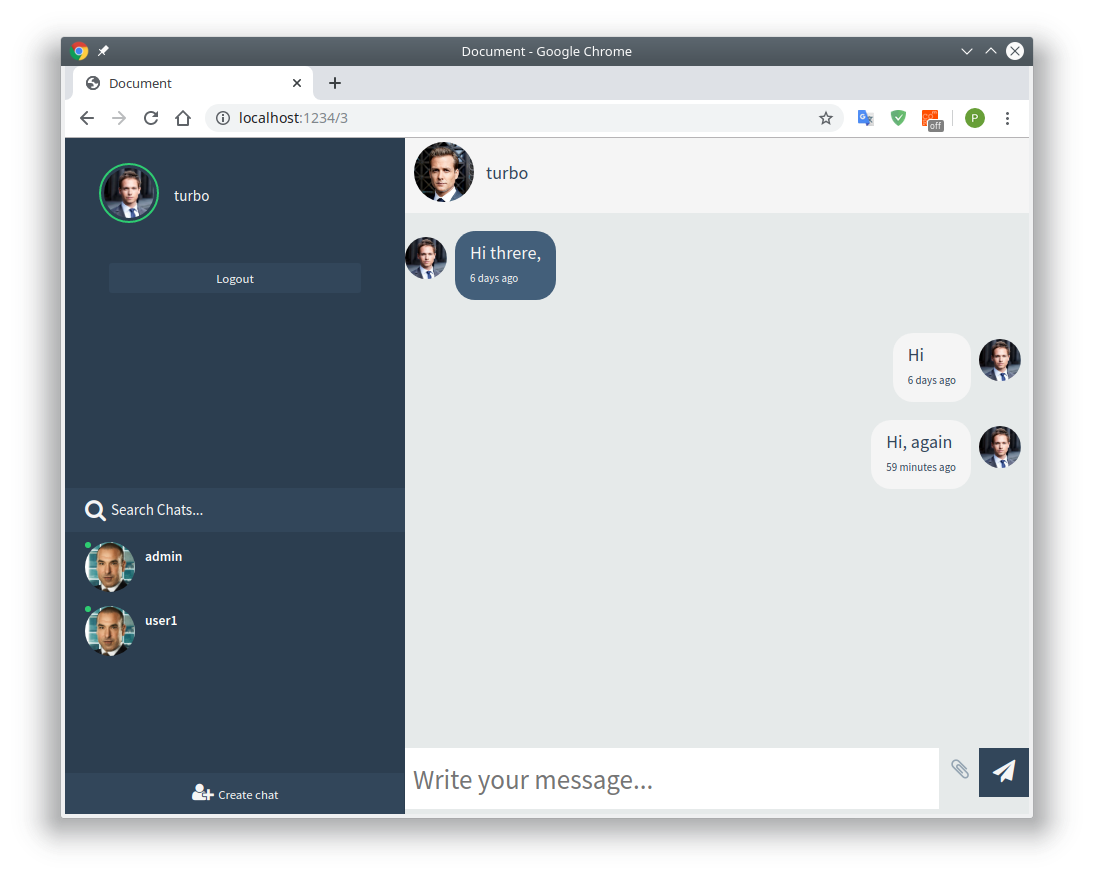
\includegraphics[scale=0.5]{Images/chatlog.png}
				\captionof{figure}{Giao diện Chat chính của ứng dụng}
			\end{center}
		Giao diện ứng dụng chia thành 3 phần, SideBar ở bên trái, Profile ở phái trên bên phải và cuối cùng là Chat ở phía bên phải.
		\item \textbf{Hệ thống tạo cuộc trò chuyện :}\\
		Có thể tạo một cuộc trò chuyện mới với các người dùng khác trong cùng hệ thống. dựa trên cơ chế REST API như hình sau : 
			\begin{center}
				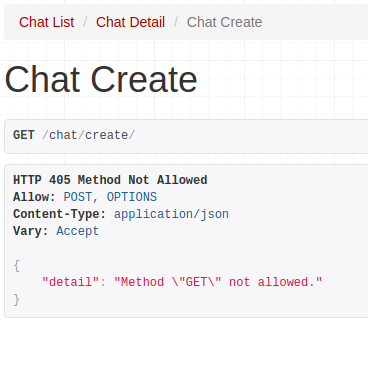
\includegraphics[scale=0.7]{Images/createchat.png}
				\captionof{figure}{Cơ chế tạo cuộc trò chuyện mới.}
				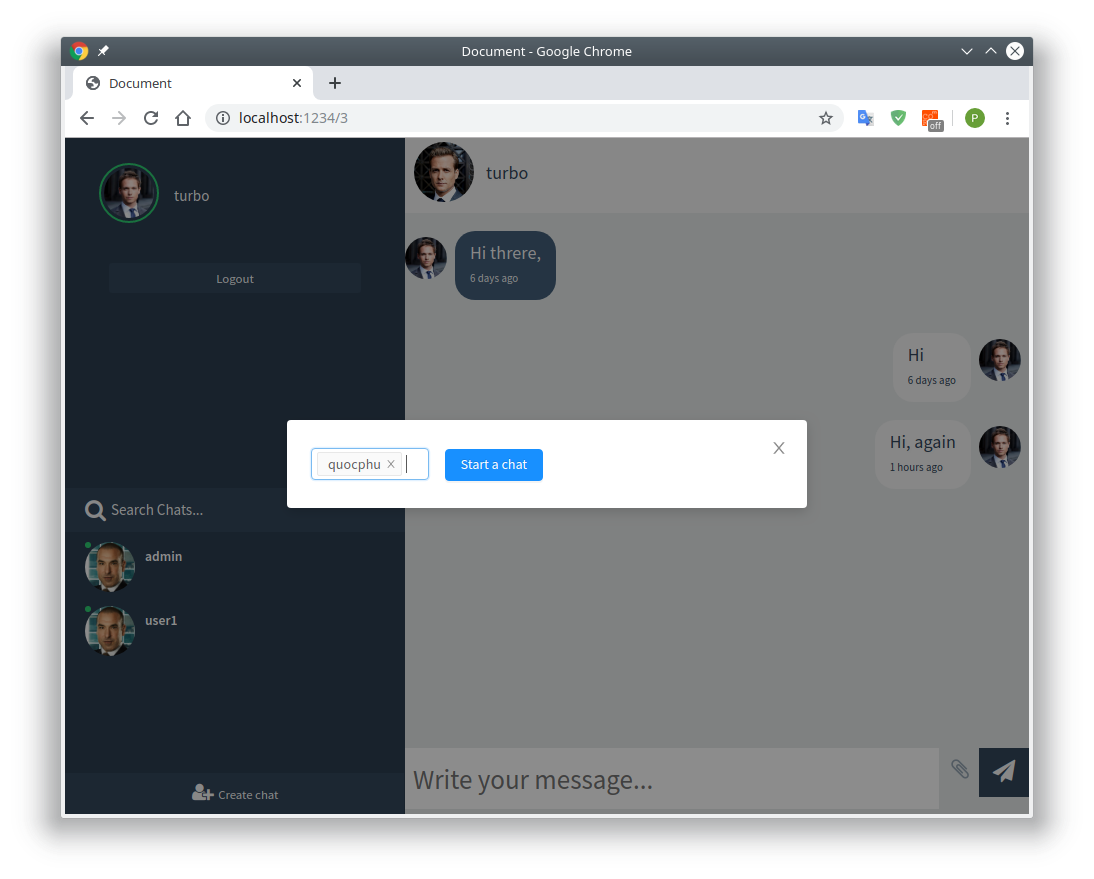
\includegraphics[scale=0.5]{Images/createchatform.png}
				\captionof{figure}{Giao diện cho việc tạo cuộc trò chuyện mới.}
			\end{center}
		\item \textbf{Hệ thống xác định trạng thái :}\\
		Xác định trạng thái hoạt động của một người dùng trong hệ thống cũng như danh sách những ngừoi dùng mà bạn đã tạo cuộc trò chuyện cùng. như hình sau :
			\begin{center}
				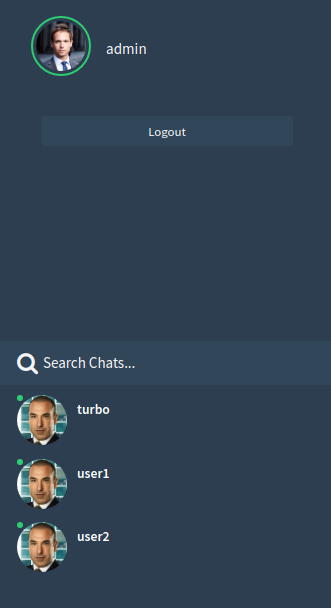
\includegraphics[scale=0.5]{Images/sidebar.png}
				\captionof{figure}{Sidebar}
			\end{center}
		\item \textbf{Hệ thống gửi file và ảnh :} \\
		Được thể hiện bằng một icon gim bấm trong phần Input-message.
			\begin{center}
				
\includegraphics[scale=0.5]{Images/chatinput.png}
			\end{center}
	\end{itemize}
	\subsection{Kiến trúc của ứng dụng : }
	Chương trình được chia là thành hai phần tách biệt : 
		\begin{itemize}
			\item Front - End : \\
			Sử dụng ReactJS cùng với Redux để hiện thực một single page application	thông qua các đặc tính của React như props hay state.
			\item Back - End : \\
			Sử dụng Django - web framework cho Python. Bởi các lợi thế từ cấu trúc phân chia theo mô hình MVC khá rõ ràng, đến vô các số tài liệu hướng dẫn. \\
			Bên trong Django nhóm sử dụng Channel - là một dự án đưa Django và mở rộng khả năng của nó vượt ra ngoài HTTP - để xử lý WebSockets, giao thức trò chuyện, giao thức IoT, v.v. Nó được xây dựng trên một đặc tả Python gọi là ASGI (Asynchronous Server Gateway Interface). Giúp Django xử lý không đồng bộ với các yêu cầu gửi đến.			
			
			
		\end{itemize}

%%%%%%%%%%%%%%%%%%%%%%%%%%%%%%%%%
\section{Mã nguồn chương trình}\label{source_code}
Cấu trúc chương trình được thể hiện như sau.
\dirtree{%
	.1 \myfolder{red}{ChatApp/}.
		.2 \myfolder{blue}{Front-end/}.
			.3 \myfolder{green}{node\_modules/}.
			.3 \myfolder{green}{src/}.
				.4 \myfolder{orange}{assets/}.
				.4 \myfolder{orange}{components/}.
				.4 \myfolder{orange}{containers/}.
				.4 \myfolder{orange}{hoc/}.
				.4 \myfolder{orange}{store/}.
				.4 \myfolder{yellow}{App.js}.
				.4 \myfolder{yellow}{index.js}.
				.4 \myfolder{yellow}{router.js}.
				.4 \myfolder{yellow}{settings.js}.
				.4 \myfolder{yellow}{websocket.js}.
			.3 \myfolder{yellow}{index.html}.
			.3 \myfolder{yellow}{package.json}.
			.3 \myfolder{yellow}{package-lock.json}.
}
\dirtree{%
	.1 \myfolder{red}{ChatApp/}.
	.2 \myfolder{blue}{Front-end/}.
	.3 \myfolder{green}{node\_modules/}.
	.3 \myfolder{green}{src/}.
	.4 \myfolder{orange}{assets/}.
	.4 \myfolder{orange}{components/}.
	.4 \myfolder{orange}{containers/}.
	.4 \myfolder{orange}{hoc/}.
	.4 \myfolder{orange}{store/}.
	.4 \myfolder{yellow}{App.js}.
	.4 \myfolder{yellow}{index.js}.
	.4 \myfolder{yellow}{router.js}.
	.4 \myfolder{yellow}{settings.js}.
	.4 \myfolder{yellow}{websocket.js}.
	.3 \myfolder{yellow}{index.html}.
	.3 \myfolder{yellow}{package.json}.
	.3 \myfolder{yellow}{package-lock.json}.
}
\end{document}

